\pdfpagewidth=8.5in
\pdfpageheight=11in

\documentclass{sig-alternate}
\usepackage[utf8]{inputenc}
\usepackage[T1]{fontenc}
\usepackage{microtype}

\usepackage{url}
\usepackage{amsmath}
\usepackage{graphicx}
\usepackage{subfigure}
\usepackage{threeparttable}
\usepackage{pdflscape}
\usepackage{array}
\usepackage{color}

\usepackage{flushend}

\clubpenalty = 10000
\widowpenalty = 10000
\displaywidowpenalty = 10000

\begin{document}

\conferenceinfo{MSR}{'15, May 16 – 17, 2015, Florence, Italy}
\CopyrightYear{2015}
\crdata{978-1-4503-2863-0/14/05}

\title{Generating the Blueprints of the Java Ecosystem}

\numberofauthors{5}

\def\aueb{\textsuperscript{*}}
\def\columbia{\textsuperscript{\ddag}}
\def\run{\textsuperscript{\dag}}

\author{
  Vassilios Karakoidas\aueb \and Dimitris Mitropoulos\columbia \and Panos Louridas\aueb \and Georgios Gousios\run \and Diomidis Spinellis\aueb\\
  \begin{tabular}{c}
   \affaddr{\aueb Dept of Management Science and Technology}\\
   \affaddr{Athens University of Economics and Business}\\
   \affaddr{Athens, Greece}\\
   \email{\{bkarak,louridas,dds\}@aueb.gr}\\
  \end{tabular}
  \centering
  \begin{tabular}{cc}
   \affaddr{\run Department of Digital Security} & \affaddr{\columbia Computer Science Department}\\
   \affaddr{Radboud University Nijmegen} & \affaddr{Columbia University}\\
   \affaddr{Nijmegen, the Netherlands} & \affaddr{New York, United States}\\
   \email{georgios@cs.ru.nl} & \email{dimitro@cs.columbia.edu}\\
  \end{tabular}
}

\maketitle
\begin{abstract}

\end{abstract}

\category{D.2.4}{Software Engineering}{Software/Program Verification}[Statistical methods]

\terms{Static Analysis, Software Ecosystems.}

\keywords{JDepend, Software Metrics, Chidamber and Kemerer.}

\section{Introduction}
\label{sec:intro}

Software metrics provide a means to extract useful and measurable information about the structure of a software system. Software development artifacts consist of digital data, many of their aspects can be easily measured. This is exemplified by the early appearance of metrics like {\sc loc} (Lines of Code) and {\sc cloc} (Comment Lines of Code). Over the years, a wealth of different metrics have appeared in the literature. Many of them, such as Chidamber and Kemerer's~\cite{CHKE94} and the metrics presented by Lorenz et al.~\cite{LOKI94} can be automatically calculated by static analysis tools.

In this paper, we present a dataset that contains popular metrics, calculated from the analysis of a large collection of Java projects. All projects were taken from the {\it Maven Central Repository}~\cite{MAVEN}. Maven is a build automation tool used mostly for Java projects. To build a software component, it dynamically downloads Java libraries and Maven plug-ins from the Maven central repository, and stores them in a local cache. The repository can be updated with new projects and also with new versions of existing projects that can depend on other versions. Note that this repository has been previously analyzed by researchers to produce relevant datasets as we discuss in Section~\ref{sec:rel}. To analyze the projects coming from this repository, we used the following tools: a) {\sc ckjm} \cite{Spi05g}, b) {\sc jd}epend~\cite{JDEPEND}, and c) {\sc clmt}~\cite{SGKL09}. All tools focus on three main aspects of a software system, namely: object-oriented design, program size, and package design.

In this paper we present: a) the construction process to obtain the collection of the metrics results that the three aforementioned tools produced for {\bf 22730} {\sc jar}s, b) our dataset and c) how researchers and practitioners can use the dataset and produce meaningful results.

\section{Dataset Construction Process}
\label{sec:data}

Maven is a build automation tool used primarily for Java projects, and it is maintained by the Apache Software Foundation~\cite{MAVEN}. To describe the software project being built, its dependencies on other libraries, and the build order Maven uses {\sc xml}. The central repository contains more than 400,000 {\sc jar}s, in a variety of languages that are all using the {\sc jvm} platform as their runtime environment. These languages include Java, Clojure, Groovy, and Scala.

\begin{figure*}
\centering
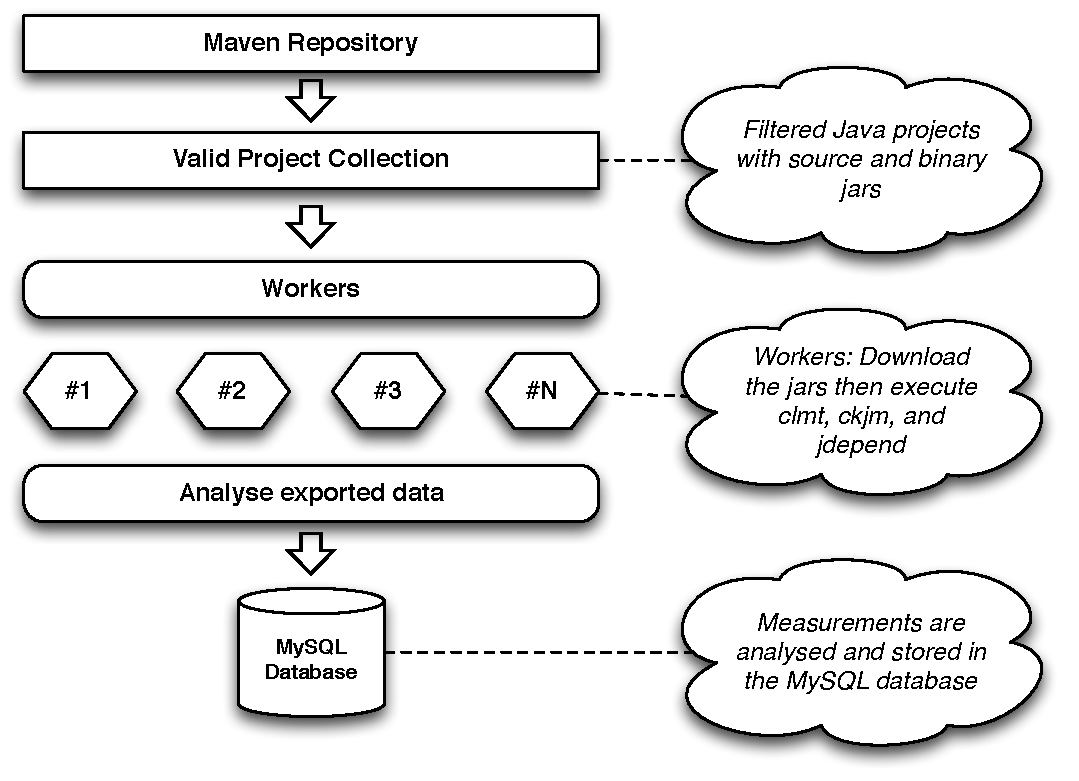
\includegraphics[scale=0.7]{import-process}
\caption{The dataset construction process}
\label{fig:dataset-construction}
\end{figure*}

The dataset construction process is illustrated in Figure~\ref{fig:dataset-construction}. Initially, a snapshot of the Maven repository was downloaded locally. The repository contains various projects and their releases. We identified only the Java projects. The repository contains several versions of each project. All versions were filtered out and only the latest was kept. Each project consists of two {\sc jar} files, one that contains a compiled version of the project and one with the source code. The projects that did not had both binary and source jars, were excluded from the experiment.

When the selection process was finished, the {\sc jars} were downloaded from the central repository and with the help of a queue, delivered into a series of workers, which executed the tools and provided a series of measurements stored in {\sc json} form. The result files were validated by scripts and then the data were imported in a MySQL database.

Table \ref{tbl:oss-size-metrics} presents several size metrics regarding the final version corpus. It included 11,365 projects, with more than 110 million lines of code. Overall the dataset contains almost 33 million unique measurements.

\begin{table}
\centering
\caption{The selected Maven projects' size metrics}
\label{tbl:oss-size-metrics}
\begin{tabular}{l r}
 \hline
\textbf{Metric} & \textbf{Value}\\
\hline
Project Count & 11,365\\
File Count & 604,821\\
Module Count & 72,302\\
Lines of Code & 110,156,703\\
Source Lines of Code & 61,246,807\\
Comment Lines of Code & 36,696,217\\
Number of Classes & 499,588\\
Number of Interfaces & 89,145\\
Number of Enumerations & 12,732\\
Measurement Count & 32,844,836\\
\hline
\end{tabular}
\end{table}

Three tools were selected to calculate the measurements.

\begin{itemize}
  \item \textbf{CKJM-ext} \textit{(ckjm)}~\cite{Spi05g} is an open source tool that was developed by Diomidis Spinellis and then extended by Marian Jureczko. It calculates many software complexity metrics, including the \textit{Chidamber and Kemmerer} set of object-oriented metrics \cite{CHKE94}. The version of the tool that we used for this experiment can be found in github~\cite{CKJM}.

  \item \textbf{JDepend} \textit{(jdep)}~\cite{JDEPEND} is a tool that analyses {\sc jar} files that contain compiled Java classes and calculates a series of design metrics.

  \item \textbf{CLMT} \textit{(clmt)}~\cite{SGKL09} stands for \textit{cross-language metric tool} and analyses the source code of several languages in order to calculate a series of size metrics.
\end{itemize}

Table~\ref{tbl:selected-metrics} presents the key metrics that are calculated and stored in the dataset. Each tool focuses on a different aspect of a software system; \textit{ckjm} focuses on object-oriented design metrics, \textit{jdepend} on package design, while \textit{clmt} focuses on program size metrics. Several metrics are calculated by more than one tool, like \textit{cyclomatic complexity}, which is calculated by both \textit{clmt} and \textit{ckjm}. Both calculations are available in the database.

A series of secondary metrics are also stored in the database. For example, a set of metrics that count the usage of specific {\sc dsl} application libraries in a software project. These are not included in the Table~\ref{tbl:selected-metrics}, since they are not commonly accepted. In Section~\ref{sec:dsl}, we describe a small experiment based on these metrics that measures the popularity of {\sc dsl} usage for the dataset anf therefore for the Java ecosystem in general.

\begin{table}
\centering
\caption{Key Metrics}
\label{tbl:selected-metrics}
\begin{tabular}{l l}
 \hline
\multicolumn{2}{l}{\textit{\textbf{Class Design}}}\\
\hline
Depth Of Inheritance Tree & \textit{ckjm}\\
Coupling Between Objects & \textit{ckjm}\\
Weighted Methods Per Class & \textit{ckjm}\\
Response For Class & \textit{ckjm}\\
Lack Of Cohesion In Methods & \textit{ckjm}\\
Number Of Children & \textit{ckjm}\\
Attribute Hiding Factor & \textit{clmt}\\
Coupling Between Methods & \textit{ckjm}\\
Average Method Complexity & \textit{ckjm}\\
Cohesion Among Methods of Class & \textit{ckjm}\\
Data Access Metric & \textit{ckjm, clmt}\\
Inheritance Coupling & \textit{ckjm}\\
Lack Of Cohesion In Methods3 & \textit{ckjm}\\
Measure Of Aggregation & \textit{ckjm}\\
Measure Of Functional Abstraction & \textit{ckjm}\\
Number of Attributes & \textit{clmt}\\
Method Hiding Factor & \textit{clmt}\\
\hline
\multicolumn{2}{l}{\textit{\textbf{Method Design}}}\\
\hline
Number of Method Parameters & \textit{clmt}\\
Number of Methods & \textit{clmt, ckjm}\\
McCabe Cyclomatic Complexity & \textit{ckjm, clmt}\\
\hline
\multicolumn{2}{l}{\textit{\textbf{Package Design}}}\\
\hline
Number of Concrete Classes & \textit{jdep}\\
Afferent Couplings & \textit{jdep, ckjm}\\
Efferent Couplings & \textit{jdep, ckjm}\\
Instability & \textit{jdep}\\
Abstractness & \textit{jdep}\\
Distance Main Sequence & \textit{jdep}\\
\hline
\multicolumn{2}{l}{\textit{\textbf{Program Size Metrics}}}\\
\hline
Number of Classes & \textit{clmt, ckjm, jdep}\\
Number of Enumerations & \textit{clmt, ckjm}\\
Number of Interfaces & \textit{clmt, ckjm}\\
Module Count & \textit{clmt, ckjm}\\
Comments Lines Of Code & \textit{clmt}\\
Lines Of Code & \textit{clmt, ckjm}\\
Source Lines Of Code & \textit{clmt}\\
Function Oriented Code & \textit{clmt}\\
DSL Usage Count & \textit{clmt}\\
File Count & \textit{clmt}\\
\hline
\end{tabular}
\end{table}

\section{Database Structure}
\label{sec:db}

Figure~\ref{fig:database-schema} illustrates the database schema. It consists of five tables; \textit{measurement}, \textit{category}, \textit{identifiers}, \textit{measurement\_type}, and \textit{project}. The central database table is \textit{measurement}, which holds the measurement values. The other tables are used for normalization.

Metrics are divided into six categories that define their scope; \textit{module}, \textit{class}, \textit{method}, \textit{code unit}, and \textit{project-wide}. These values are stored in \textit{category} database table.

The descriptive names for each metric are stored in the \textit{measurement\_type} database table. There are 65 metrics available in the dataset. The names are composed by the actual metric name and the tool that was used to calculate them e.g. \textit{McCabe\_clmt} denotes that the metric name is the McCabe cyclomatic complexity from the \textit{clmt} tool, while \textit{McCabe\_ckjm} means that it is the same metric calculated by the \textit{ckjm} tool.

Filenames, methods, classes and package names along with other identifiers are stored in the \textit{identifiers} table. Note that each measurement has a related filename and a related identifier that points to a software element e.g. the \textit{afferent coupling} metric for the module in the directory ``com/scalagent/jmx'' is related with the identifier \textit{com.scalagent.jmx}.

Finally, the database table \textit{project} contains the related project identifiers, extracted from the maven repository.

\begin{figure*}
\centering
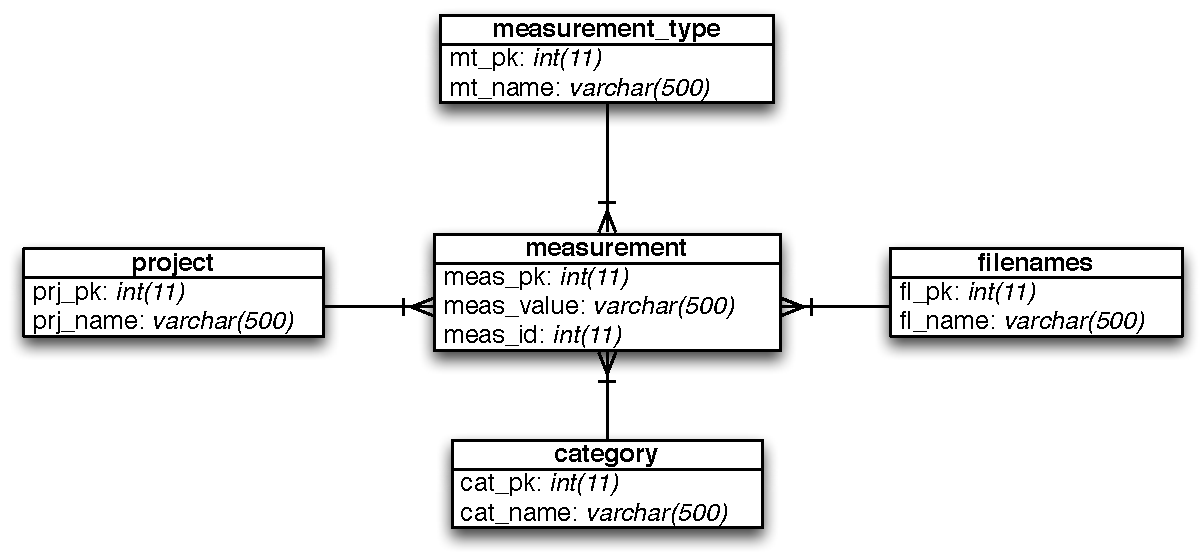
\includegraphics[scale=0.7]{database-schema}
\caption{The database schema}
\label{fig:database-schema}
\end{figure*}

\section{Research Opportunities}
\label{sec:research-opportunities}

The measurements provided by this dataset, can be exploited in many

\section{Experimenting with the Dataset}
\label{sec:dsl}

Along with the

The methodology was the following: A set of standard {\sc dsl} application libraries was identified, and the source was scanned for specific \textit{import} statements e.g. \textit{java.util.regex}, which indicated that the standard package that implements regular expressions was used, thus regular expressions were used. If a package is detected in the source code, then the project will be tagged that it uses one (1) {\sc dsl}. Consequently, if a project has {\sc dsl} count four (4), then it means that four (4) different application libraries were detected during the source code scan. Table \ref{tbl:dsl-list} lists the selected {\sc dsl}s application libraries. Note that all these libraries are included as part of the Java {\sc sdk}.

\begin{table}
\centering
\caption{List of selected DSL application libraries}
\label{tbl:dsl-list}
\begin{tabular}{l l}
 \hline
\textbf{DSL} & \textbf{Java Package}\\
\hline
Regular Expressions & \verb|java.util.regex|\\
XML & \verb|javax.xml|, \verb|org.w3c| and \verb|org.xml|\\
SQL & \verb|java.sql| and \verb|javax.sql|\\
XPath & \verb|java.xml.xpath|\\
XSLT & \verb|javax.xml.transform|\\
RTF & \verb|javax.swing.text.rtf|\\
HTML & \verb|javax.swing.text.html|\\
\hline
\end{tabular}
\end{table}

The initial goal of this experiment was to provide quantifiable results that are indicative regarding the usage of each {\sc dsl}, thus only files containing Java code were taken into account. Build files or other resources that may contain {\sc dsl}s were not included. One final assumption was also made; if {\sc xpath} or {\sc xslt} were found in the source code, then the project would be marked that it also uses {\sc xml}, since those two languages are used for query and transformations on {\sc xml} {\sc dom} trees.

\begin{table}
\centering
\caption{Popular DSL Usage Combinations}
\label{tbl:dsl-top-usage}
\begin{tabular}{l r}
 \hline
\textbf{DSLs} & \textbf{Count}\\
\hline
XML & 1,561\\
Regex & 909\\
SQL & 493\\
XML, XSLT & 475\\
Regex, XML, XSLT & 158\\
Regex, XML & 303\\
SQL, XML & 162\\
Regex, SQL & 116\\
Regex, SQL, XML, XSLT & 80\\
Regex, SQL, XML & 71\\
SQL, XML, XSLT & 54\\
XML, XPath & 50\\
XML, XPath, XSLT & 39\\
Regex, XML, XPath, XSLT & 38\\
HTML & 23\\
Regex, XML, XPath & 20\\
Regex, SQL, XML, XPath, XSLT & 18\\
SQL, XML, XPath, XSLT & 11\\
HTML, Regex, XML & 10\\
HTML, XML & 10\\
\hline
\end{tabular}
\end{table}

\section{Limitations}
\label{sec:limit}

This dataset followed a narrow selection process, identifying and analysing only projects that were written in Java and had the source code and the binary jar available in the repository. The latter reduced significantly the number of projects that were analysed, since many of them provided only the binary jar. Since only \textit{clmt} analyses the source code, this ended in drastically reduction of measurements that were exposing object-oriented and package design issues.

In addition, only one version was analysed per project. Usually, the latest, which was replaced by a prior version, only if it was violating the aforementioned selection process. This decision rendered the dataset unusable, for research focused on evolutionary changes of a software project.

\section{Related Work}
\label{sec:rel}

The Maven ecosystem has been previously analyzed by Raemaekers et al.~\cite{RDV13} to produce the {\it Maven dependency dataset}. Apart from basic information like individual methods, classes, packages and lines of code for every {\sc jar}, this dataset also includes a database with all the connections between the aforementioned elements.

In reference \cite{MKLGS14}, Mitropoulos et al. also experimented in a similar way, by running the FindBugs~\cite{HP04} tool on a large part of the maven repository. Our work differs from these two approaches since it presents the metrics calculated by the three aforementioned tools; \textit{ckjm}, \textit{jdepend}, and \textit{clmt}.

\section{Conclusions}
\label{sec:conc}

This dataset is a source of measurements for a large selection of projects, covering the basic scopes of software design, with metrics covering from program size to object-oriented design. In the future, we plan to keep an updated version of the dataset, by analysing the new additions and updates of the maven repository. In addition, our selection process should be more elastic, allowing the participation of projects, that cannot be analysed by all the tools, due to source code unavailability.

Finally, all versions for each project should also be included, allowing researchers to include the dataset to approaches that focusing on the evolutionary aspect of a software package.

\section{Availability}

The dataset and the source code of this publication, along with some utility scripts are available at \url{https://github.com/bkarak/data_msr2015}.

\bibliographystyle{abbrv}
\bibliography{msr}

\end{document}
